\chapter{Objetivos y metodología}\label{chap:objetivos}
Una vez expuestas las motivaciones y contexto del proyecto, en este capítulo se detallan los objetivos y la metodología empleada. 

\section{Objetivos}
El propósito de este proyecto es la extensión y mejora de la herramienta docente basada en el simulador \textit{WebSim} que está orientada a facilitar el aprendizaje de programación y robótica. Para cumplir ese propósito se han fijado varios subobjetivos:
\begin{itemize}
    \item Añadir soporte para \textit{drone} en la plataforma, incluyendo tanto su simulación realista en su apariencia visual y en comportamiento físico como la infraestructura para que sea programable desde fuera del simulador.
        
    \item Añadir teleoperadores para que los robots se puedan controlar manualmente sin necesidad de programarlos. De esta manera se facilita la labor de los desarrolladores al poder probar el entorno y los sensores del robot de manera sencilla.
    
    \item Incluir más ejercicios didácticos sobre \textit{WebSim} que aprovechen los distintos \textit{robots} soportados por la plataforma y que sean vistosos, motivantes, asequibles y desafiantes para los estudiantes. Esto implica elaborar escenarios y archivos de configuración para los distintos ejercicios. 

    \item Incluir \textit{ejercicios competitivos} de tal manera que dos usuarios puedan programar sobre el mismo escenario. Este objetivo también incluye crear un evaluador automático para puntuar la eficacia del comportamiento de cada robot. Con ello se pretende fomentar la ``\textit{gamificación}'' de la plataforma educativa.
    
\end{itemize}
\section{Metodología}
\label{sec:metodologia}

Para el desarrollo del proyecto se han hecho reuniones semanales con el tutor del TFG en las que se elaboraba un plan de trabajo para la semana y se revisaban las tareas concluidas. Cuando era necesario tener un desarrollo terminado, se aumentaba la frecuencia de las reuniones.\newline
Este tipo de trabajo se asemeja mucho a la metodología \textit{extreme programming}. Esta forma de trabajar es una metodología \textit{agile} con el objetivo de conseguir un código de calidad y flexible y mejorar la productividad. Es un método muy útil para proyectos con requisitos cambiantes porque hace énfasis en la adaptabilidad. 
Para su cumplimiento son fundamentales la comunicación y realimentación con el resto de integrantes del equipo. Para ello se ha utilizado la herramienta \textit{Slack}\footnote{\url{https://slack.com/}} en la que los desarrolladores están en contacto en todo momento.

Se ha elaborado un \textit{blog} en el que se describía la evolución de las tareas semanales. Dicha evolución se registra en el \textit{README.md} del repositorio habilitado para este TFG\footnote{\url{https://github.com/RoboticsLabURJC/2019-tfg-ruben-alvarez}}.
Para el desarrollo de este proyecto se ha utilizado otro repositorio en el que se desarrolla el software principal del proyecto\footnote{\url{https://github.com/jderobot-hub/kibotics-websim}} y en el que participa un equipo de seis personas. 

En el repositorio principal, la metodología de trabajo durante el proyecto ha consistido en crear incidencias (\textit{issues}) de alguna tarea en específico (con el fin de solucionar problemas o añadir funcionalidad) y para cerrarla se creaba una rama (\textit{branch}) realizando después un parche (\textit{pull request}) para fusionarlo con la rama principal y así arreglar la incidencia. Se sigue esta metodología para registrar de forma limpia los cambios realizados por los diferentes desarrolladores que trabajan sobre el repositorio y, en caso de ser una modificación importante, solicitar la supervisión de otro desarrollador para integrarla. En la figura \ref{fig:github} se puede observar gráficamente una cronología de las ramas del repositorio durante medio mes de trabajo.

 \begin{figure}[H]
    \centering
    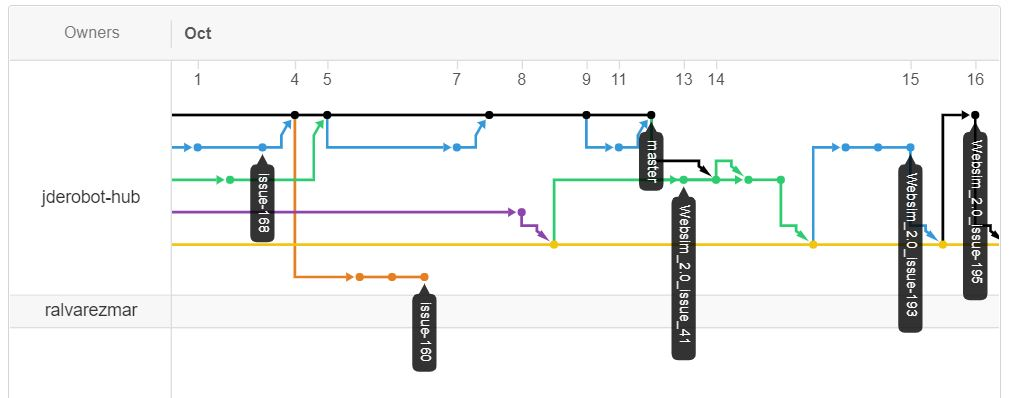
\includegraphics[width=0.9\textwidth]{img/github.jpg}
    \caption{Representación gráfica de las ramas del proyecto} \label{fig:github}
\end{figure}

En el repositorio del \textit{blog} se realizó una copia (\textit{fork}) para trabajar directamente sobre la cuenta personal de \textit{GitHub}\footnote{\url{https://github.com/ralvarezmar/2019-tfg-ruben-alvarez}}. De esta manera, en primera instancia se suben los cambios al repositorio personal y, cuando hay progresos importantes, se suben todos los cambios al repositorio original. Para automatizar esta tarea se ha realizado un \textit{script} de \textit{shell} en el que el primer argumento es el mensaje del \textit{commit} y, si se escribe \textit{'-t'} después de este, se realiza la subida al repositorio copiado y al original.\newline

\begin{lstlisting}[language=bash, caption=\textit{Script} para subir código a \textit{GitHub}]
#!/bin/sh
if [ $# -gt 2 ]
then
	echo "usage: $1 " 1>&2
	exit 1
fi
git add .
git commit -m "$1"
git push
if [ "$2" = "-t" ]
then
	git push upstream
fi
\end{lstlisting}

\section{Plan de trabajo}
\label{sec:plan}

Se ha establecido un plan de trabajo dividido en fases para afrontar los objetivos previstos: 
\begin{itemize}
    \item Fase 1: Estudio de \textit{A-Frame} y de \textit{Websim}. Periodo de aprendizaje y familiarización con el entorno en el que se va a trabajar. 
    \item Fase 2: Desarrollo de soporte a \textit{drones} y nuevos modelos. Incluye la ampliación de los drivers y creación de bloques de \textit{Scratch} que se apoyan en esos \textit{drivers}.
    \item Fase 3: Desarrollo de teleoperadores web. Incorpora el diseño de un frontal para seleccionar teleoperador entre los modelos disponibles de \textit{WebSim}.
    \item Fase 4: Ejercicios individuales. Se lleva a cabo el desarrollo, creación, prueba de nuevos escenarios, nuevos enunciados y la programación de soluciones de referencia. 
    \item Fase 5: Ejercicios competitivos y evaluadores automáticos. Comprende la creación de escenarios, nuevos modelos, el diseño de cada evaluador y la lógica para su correcto funcionamiento. 
\end{itemize}